\chapter{Filter}
\label{ch:concept}
\section{Allgemeines}
Neben Oszillatoren wie VCO und LFO stellen der Filter ein wichtiges Element der Klangsynthese dar.
In diesem Kapitel wird eine Realisierungsform eines spanungsgesteuerten Filters VCF vorgestellt. 
Grundsätzlich kann ein Filter bestimmte Frequenzanteile eines Signals ungehindert passieren lassen, während andere Anteile
abgeschwächt werden.
Man unterscheidet zwischen dem sogennanten Durchlassbereich, Übergansbereich und Sperrbereich.

\begin{figure}[h]
	\centering
	\setlength{\fboxsep}{1pt} %Abstand der Linien zur Abbildung
	\setlength{\fboxrule}{1pt} %Dicke der Linie
	\fbox{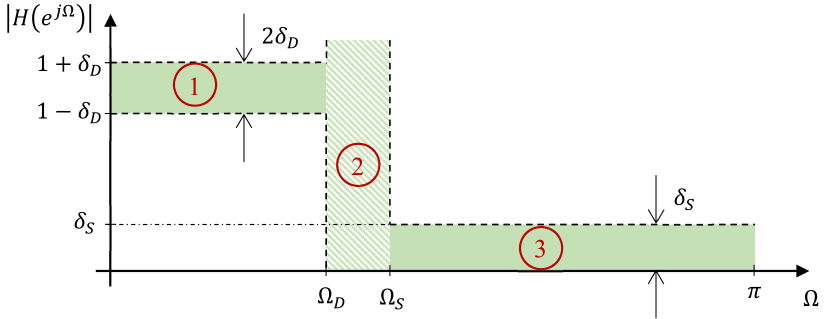
\includegraphics[width=0.5\textwidth]{figures/toleranzschema.png}}
	\caption{Frequenzgang eines digitalen Filters}
	\label{fig:toleranzschema}
\end{figure}
Abbildung \ref{fig:toleranzschema} zeigt ein schematisches Schaubild für einen digitalen Filterentwurf, der hier analog adaptiert werden kann.

\textbf{Durchlassbereich:}\\
Der Durchlassbereich wird bis zur Grenzfrequenz $f_{3dB}$ (engl. Cut-Off Frequency) definiert.
Beim VCF kann diese Grenzfrequenz mit einer Steuerspannung und einem Potentiometer verändert werden. \\

\textbf{Übergangsbereich:}\\
Im Übergansbereich will man grundsätzlich meist eines steile Flanke realisieren. Die Flankensteilheit wird normalerweise in dB/Dec bzw. dB/Oct angegeben.
Steile Flanken können ohne weitere tiefergehende Entwurfsmethoden (z.B Cauer, Tschebychef o.Ä) nur mit einer höheren Filterordnung realisiert werden.
Im Übergangsbereich ist außer der Flankensteilheit noch das Resonanzverhalten interessant. Um die Resonanzfrequenz $f_r$ werden Frequenzanteile um einen Faktor Q (Güte) erhöht.  
Es gilt: 
\begin{equation}  \label{eq:1}
  |H(f_r)| = H_0 \cdot Q
\end{equation}
Für Audiofilter hat das Resonanzverhalten eine große Bedeutung, da dieser Fall besonders voll und interessant klingt.\\
\\
\textbf{Sperrbereich:}\\
Frequenzanteile, die sich im Sperrbereich befinden werden werden dann je nach Frequenzwert mit der entsprechenden Flankensteilheit abgeschwächt.


\section{Schaltplan}
Das Eingangssignal geht über die Audiobuchse J3 über einen Eingangskondensator C2, der den DC-Offset des Signals herausfiltert in den Eingang des OPVs.
Der OPV hat eine Leerlaufverstärkung im Durchlassbereich von $-\frac{R2}{R1+R7} = 0.3 = 20 log_{10}(0.3) = -10.456 dB$. Dieser Wert wurde so gewählt,
um bei starker Resonanz keine Eingänge von nachfolgenden Modulen zu zerstören. Das eigentliche Tiefpass-Verhalten wird durch die Kondensatoren C3 und C4, sowie die Widerstände R3 und R4 realisiert. 
Die Grenzfrequenz kann über den einen JFET justiert werden. Dieser fungiert als spanungsgesteuerter Widerstand. Der Drain des JFET liegt Potenzialmäßig zwischen C3 und C4 bzw. R3 und R4 und Ground.
Somit kann das Potenzial dieses Knotens Nieder- bis Hochohmig Richtung Ground gezogen werden. Bei einer Niederhomigen Verbindung (JFET durchgeschalten mit $R_{on} = 100\Omega$) ist die Grenzfrequenz maximal.\\
Mit dem Potentiometer VR2 kann zusätzlich das Resonanzverhalten eingestellt werden. Je niederhomiger der Widerstandswert, desto höher die Resonanzüberhöhung.
Somit muss der JFET in einem sinnvollen Bereich angesteuert werden, indem er auch als Widerstand fungiert. Laut Datenblatt fängt der J113 ab -3V $U_{GS}$ langsam das Leiten an und ist bei -0.5V voll durchgeschalten.
Tests mit dem Steckbrett haben gezeigt, dass der JFET erst bei -1.3V das Leiten anfängt. Es muss also eine Steuerspannung in einem Bereich von +- 4V auf einen Spannungsbereich von -0.5V bis -1.3V abgebildet werden.
Das geschieht mit der Verstärkerschaltung um den 2. OPV. Da das genaue Dimensionieren hier Formelmäßig viel zu komplex wäre, wurde ein Trimmpotentiometer R10 eingesetzt, um den Verstärkungsfaktor des OPVs einzustellen
und somit die Steuerspannung CV auf den Spannungsbereich des JFETs abzustimmen.
Zuätzlich werden die Steuerspannungen CV1 und CV2 noch über R15 über R16 mit einem Offset VR1 gemischt.
Ist keine Steuerspannung angeschlossen kann über VR1 über den oben genannten Mechanismus die Grenzfrequenz des Filters eingestellt werden. \\
\\
Insgesamt ergiebt sich mit der Bauteildimmensionierung ein Tiefpassfilter 2. Ordnung mit einer Flankensteilheit von -20dB/Dec im Sperrbereich. Die Grenzfrequenz kann über das Potentiometer VR1 oder den CV-Eingang in einem Bereich von 100Hz - 6kHz eingestellt werden.

\begin{figure}[h]
	\centering
	\setlength{\fboxsep}{1pt} %Abstand der Linien zur Abbildung
	\setlength{\fboxrule}{1pt} %Dicke der Linie
	\fbox{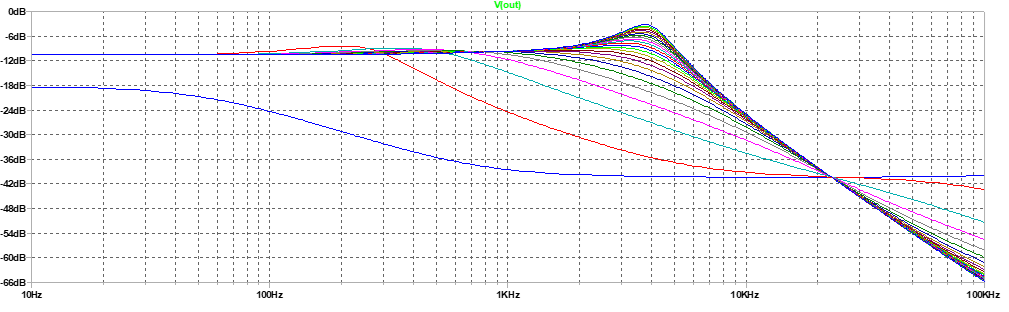
\includegraphics[width=1\textwidth]{figures/cv_sweep.png}}
	\caption{Frequenzgang des Filters bei CV-Sweep CV1 -4V bis +4V}
	\label{fig:toleranzschema}
\end{figure}

\begin{figure}[h]
	\centering
	\setlength{\fboxsep}{1pt} %Abstand der Linien zur Abbildung
	\setlength{\fboxrule}{1pt} %Dicke der Linie
	\fbox{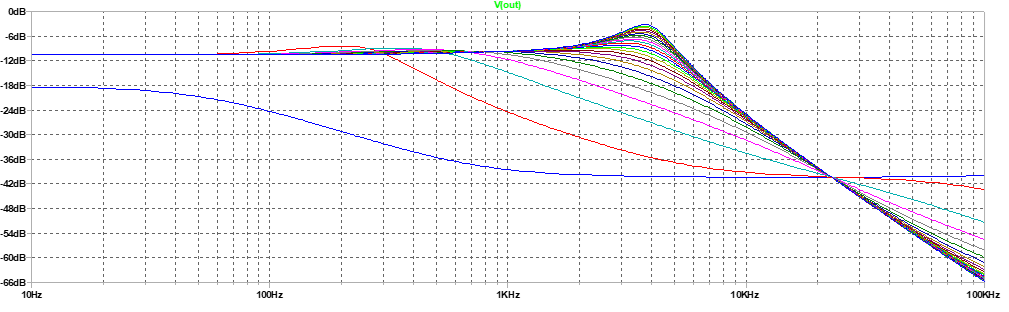
\includegraphics[width=1\textwidth]{figures/cv_sweep.png}}
	\caption{Frequenzgang des Filters bei Potentiometer-Sweep VR1 0 bis 100k$\Omega$}
	\label{fig:toleranzschema}
\end{figure}

Hier ist auch gleich eine Schwäche des Filters sichtbar. Trotz des Maximalen Potentiometer-Werts von VR2 ("Resonanz-Poti") geht der Frequenzgang
zwischen 3kHz und 4kHz in eine Resonanz (ca. 6dB Überhöhung $\rightarrow Q = 2$). Die Einstellungen Resonanz und Grenzfrequenz können also nicht komplett unabhängig von einander eingestellt werden.

\begin{figure}[h]
	\centering
	\setlength{\fboxsep}{1pt} %Abstand der Linien zur Abbildung
	\setlength{\fboxrule}{1pt} %Dicke der Linie
	\fbox{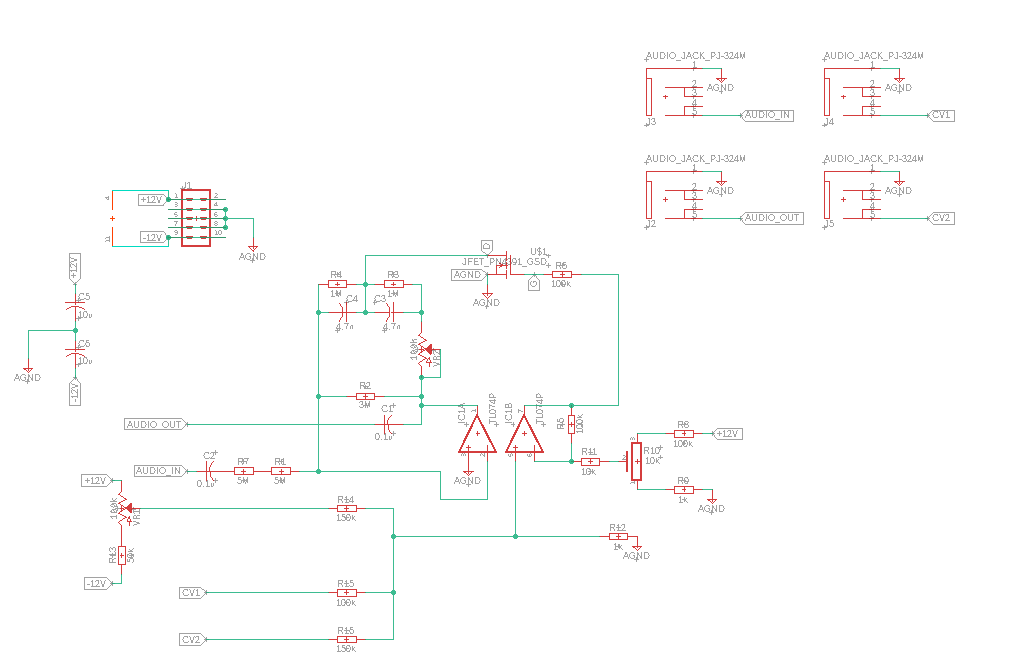
\includegraphics[width=1\textwidth]{figures/Schaltplan_VCF_verbessert.PNG}}
	\caption{Scaltplan des VCF}
\end{figure}
\newpage
\section{Platine}
\begin{figure}[h]
	\centering
	\setlength{\fboxsep}{1pt} %Abstand der Linien zur Abbildung
	\setlength{\fboxrule}{1pt} %Dicke der Linie
	\fbox{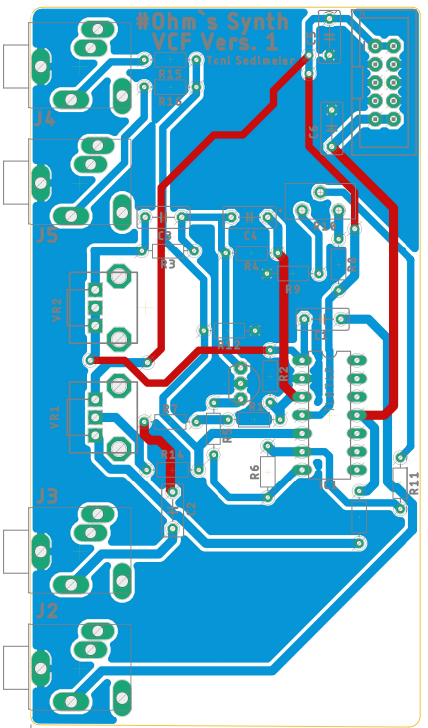
\includegraphics[width=0.3\textwidth]{figures/layout_vcf.png}}
	\caption{Platinen-Layout des VCF}
\end{figure}

\section{Mechanischer Aufbau}
\begin{figure}[h]
	\centering
	\setlength{\fboxsep}{1pt} %Abstand der Linien zur Abbildung
	\setlength{\fboxrule}{1pt} %Dicke der Linie
	\fbox{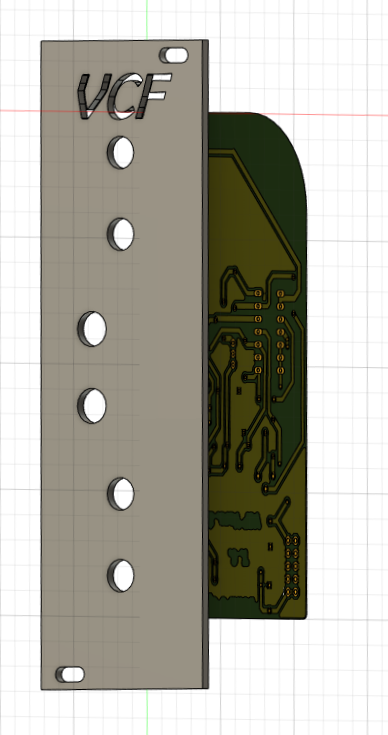
\includegraphics[width=0.7\textwidth]{figures/VCF_Abdeckung.png}}
	\caption{3D-Darstellung der VCF-Frontplatte}
\end{figure}
